
\begin{figure}
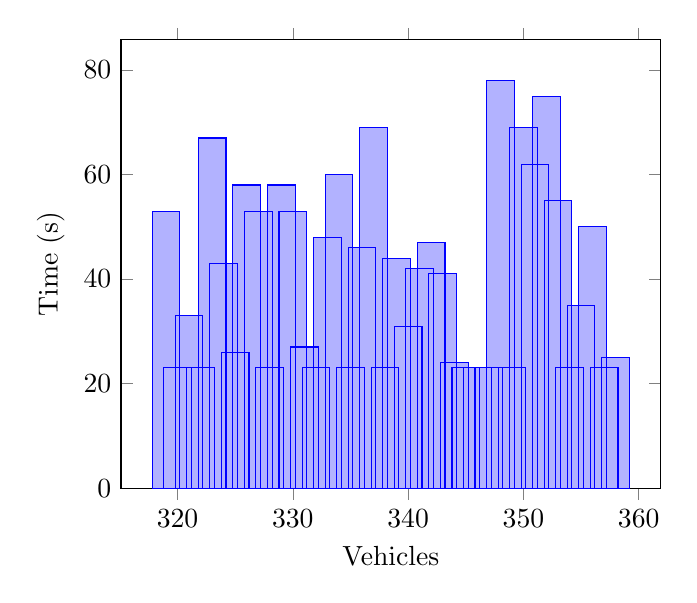
\begin{tikzpicture}
\begin{axis}[
legend style={anchor=west},
xlabel=Vehicles,
ylabel=Time (s),
ymin=0,
ybar,
]
\addplot coordinates {
(346, 23)
(347, 23)
(340, 31)
(341, 42)
(342, 47)
(343, 41)
(345, 23)
(339, 44)
(338, 23)
(335, 23)
(334, 60)
(337, 69)
(336, 46)
(331, 27)
(330, 53)
(333, 48)
(332, 23)
(344, 24)
(348, 78)
(349, 23)
(356, 50)
(322, 23)
(323, 67)
(320, 23)
(326, 58)
(327, 53)
(325, 26)
(328, 23)
(329, 58)
(319, 53)
(357, 23)
(355, 35)
(354, 23)
(353, 55)
(352, 75)
(351, 62)
(350, 69)
(358, 25)
(321, 33)
(324, 43)
};

\end{axis}
\end{tikzpicture}
\label{tik:time:100:9}
\caption{100 percent diving with GSC on route $9$}
\end{figure}
